


In order to extract a critical temperature for the quenching of pairing 
correlations from our data, we have to be careful, not to depend too much on 
the extrapolation of $\rho$. An inspection of Fig.~\ref{fig:leveldensity} shows
that the level density is roughly composed of two components as proposed by 
Gilbert and Cameron \cite{GC65}: (i) a low energetic part; approximately a 
straight line in the log plot, and (ii) a high energetic part including the 
theoretical Fermi gas extrapolation; a slower growing function. For 
illustration, we construct a simple level density formula composed of a 
constant temperature level density part with $\tau$ as temperature parameter, 
and a Fermi gas expression 
\begin{equation}
\rho(E)\propto\left\{\begin{array}{cc}\eta\exp(E/\tau)&{\mathrm{for}}\ E\leq
\varepsilon\\
E^{-3/2}\,\exp(2\sqrt{aE})&{\mathrm{for}}\ E>\varepsilon
\end{array}\right.,
\label{eq:composit}
\end{equation}
where $\eta=\varepsilon^{-3/2}\,\exp(2\sqrt{a\varepsilon}-\varepsilon/\tau)$ 
accounts for continuity at the energy $E=\varepsilon$. If we also require the 
slopes to be equal at $\varepsilon$, the level density parameter $a$ is 
restricted to
\begin{equation}
a=\left(\frac{\sqrt{\varepsilon}}{\tau}+\frac{3}{2\,\sqrt{\varepsilon}}
\right)^2.
\label{eq:condition}
\end{equation}

Figure~\ref{fig:simulation} shows the heat capacity evaluated in the canonical 
ensemble with the level density function of Eq.~(\ref{eq:composit}) and 
$\tau^{-1}=1.7$~MeV$^{-1}$. The left hand part simulates a pure Fermi gas 
description, i.e.\ the case $\varepsilon=0$, assuming a level density parameter
$a=20$~MeV$^{-1}$. One can see that a pure Fermi gas does not give rise to the 
characteristic S-shape of the heat capacity as in Fig.~\ref{fig:heatcapacity}.
The right hand part simulates the experiments, where $\varepsilon=5$~MeV and 
$a$ fulfills Eq.~(\ref{eq:condition}), i.e.\ again $a=20$~MeV$^{-1}$. The 
characteristic S-shape emerges. 

Therefore, our method to find $T_c$ relies on the assumption that the lower 
energetic part of the level density can be approximately described by a 
constant temperature level density. Calculating $\langle E(T)\rangle$ and
$C_V(T)$ within the canonical ensemble for an exponential level density gives 
$T^{-1}=\langle E(T)\rangle^{-1}+\tau^{-1}$ and 
\begin{equation}
\label{eq:Tc}
C_V(T)=(1-T/\tau)^{-2}.
\end{equation}
Thus, plotting $T^{-1}$ as function of $\langle E(T)\rangle^{-1}$ one can  
determine $\tau$ from Fig.~\ref{fig:critical}. The quantity $\tau$ is then 
identified with the critical temperature $T_c$, since $C_V(T)$ according to 
Eq.~(\ref{eq:Tc}) exhibits a pole at $\tau$ and the analogy with the definition
of $T_\lambda$ in the theory of superfluids becomes evident. The $C_V(T)$ curve
of Eq.~(\ref{eq:Tc}) with $T_c=\tau$ using the extracted critical temperatures 
for the four nuclei is shown as dashed-dotted lines in 
Fig.~\ref{fig:heatcapacity}. This simple analytical expression with only one 
parameter $T_c$ fits the experimental data up to temperatures of $\sim$0.4~MeV.
The critical temperature itself is marked by the vertical lines. The extracted 
$T_c$ is rather close to the estimate of $T_c$ represented by the arrows.
The extracted values are $T_c=$ 0.52, 0.49, 0.50 and 0.49 MeV for the 
$^{161,162}$Dy and $^{171,172}$Yb nuclei respectively, which are somehow 
delayed compared to a degenerated BCS model with $T_c=0.5\,\Delta$ yielding 
$T_c\sim$ 0.48, 0.46, 0.41 and 0.38~MeV for the respective nuclei, where 
$\Delta$ is calculated from neutron separation energies \cite{FS96}. 

We will now discuss how sensitive the extracted critical temperature is with
respect to the extrapolation, and we will give an estimate of the uncertainty
of the extracted critical temperatures. In the fit in Fig.~\ref{fig:critical},
we use only energies from $\langle E\rangle\sim$ 0.5--2~MeV. This corresponds
to energies in the level density curves up to $E_n\sim$6~MeV according to 
Eq.~(\ref{eq:energy}). Also in Fig.~\ref{fig:heatcapacity}, the interval where
Eq.~(\ref{eq:Tc}) fits the experimental data is $T\sim$0--0.4~MeV. This
corresponds to energies in the level density curves up to $E_n\sim$8~MeV. Thus,
the extracted critical temperature does only depend weakly on the actual 
extrapolation of $\rho$ curve. Also the S-shape of the $C_V(T)$ curve depends 
only on the fact, that the nuclear level density develops somehow as a Fermi 
gas expression at energies somewhere above the neutron binding energy. However,
the actual values of the $C_V(T)$ curve above $T\sim$0.5~MeV do depend on the 
specific extrapolation chosen.

With respect to $T_c$, the extrapolation is only important for determining the 
parameters $A$ and especially $\alpha$ of Eq.~(\ref{eq:transformation}). We can
therefore estimate the error of $T_c$ by 
\begin{equation}
\left(\frac{\Delta E\,\Delta T_c}{T_c^2}\right)^2=
\left(\frac{\Delta a\,\Delta U}{2\,\sqrt{aU_n}}\right)^2+
\left(\frac{\Delta D}{D}\right)^2+2\,(0.05)^2,
\end{equation}
where $\Delta E$ is the energy difference between the upper and lower energy
where $A$ and $\alpha$ are determined. $\Delta a$ is the uncertainty of the 
level density parameter, $\Delta U$ is the energy difference between the 
neutron binding energy and the upper point where $A$ and $\alpha$ are 
determined, $U_n$ is the (shifted) neutron binding energy. $D$ and $\Delta D$ 
are the neutron resonance spacing and its error. The errors of 5\% are added in
order to account for the two fitting procedures, one fitting $A$ and $\alpha$ 
the other fitting $T_c$, both with an uncertainty of some 5\%. Using a very 
conservative estimate of $a\approx 17.5(6.0)$~MeV$^{-1}$, $U_n<8$~MeV, 
$\Delta U<3$~MeV, $D/\Delta D<0.2$ and $\Delta E>4.5$~MeV, we obtain 
$\Delta T_c<0.04$~MeV. This yields a maximum error of $T_c$ of some 8\%. It is
also important to notice, that due to the strong smoothing in 
Eq.~(\ref{eq:energy}), the errors of the experimental level density curves are
negligible in our calculation.

In conclusion, we have seen a fingerprint of a phase transition in a finite 
system for the quenching of pairing correlations as a whole, given by the 
S-shape of the canonical heat capacity curves in rare earth nuclei. For the 
first time the critical temperature $T_c$ at which pair correlations in rare 
earth nuclei are quenched, has been extracted from experimental data. The 
reminiscence of the quenching process is distributed over a 6~MeV broad 
excitation energy region, which is difficult to observe and interpret in the 
microcanonical ensemble. Simple arguments show that the peak in the heat 
capacity arises from two components in the level density; a constant 
temperature like part and a Fermi gas like part. It would be very interesting 
to compare our results with SMMC calculations performed for a narrow spin 
window.

The authors are grateful to E.A.~Olsen and J.~Wikne for providing the excellent
experimental conditions. We thank Y. Alhassid for several interesting 
discussions. We wish to acknowledge the support from the Norwegian Research 
Council (NFR). 

\begin{references}
\bibitem{SY63}M. Sano and S. Yamasaki, Prog.\ Theor.\ Phys.\ \bf 29\rm, 397 
(1963) 
\bibitem{Go81}A.L. Goodman, Nucl.\ Phys.\ A\bf 352\rm, 45 (1981) 
\bibitem{FS76}A. Faessler \sl et al.\rm, Nucl.\ Phys.\ A\bf 256\rm, 106 (1976) 
\bibitem{DK95}T. D{\o}ssing \sl et al.\rm, Phys.\ Rev.\ Lett.\ \bf 75\rm, 1276
(1995)  
\bibitem{MB99}E. Melby \sl et al.\rm, Phys.\ Rev.\ Lett.\ \bf 83\rm, 3150 
(1999)
\bibitem{Ng90}Nguyen Dinh Dang, Z. Phys.\ \bf A335\rm, 253 (1990)
\bibitem{LJ93}G.H. Lang, C.W. Johnson, S.E. Koonin, and W.E. Ormand, Phys.\ 
Rev.\ \bf C48\rm, 1518 (1993)
\bibitem{KD97}S.E. Koonin, D.J. Dean, and K. Langanke, Phys.\ Rep.\ \bf 278\rm,
1 (1997) 
\bibitem{Or97}W.E. Ormand, Phys.\ Rev.\ \bf C56\rm, R1678 (1997) 
\bibitem{WK98}J.A. White, S.E. Koonin, and D.J. Dean, Phys.\ Rev.\ \bf C \rm 
(to be published)
\bibitem{RH98}S. Rombouts, K. Heyde, and N. Jachowicz, Phys.\ Rev.\ \bf C58\rm,
3295 (1998)
\bibitem{AL99}Y. Alhassid, S. Liu, and H. Nakada, Phys.\ Rev.\ Lett.\ \bf 
83\rm, 4265 (1999)
\bibitem{Al99}Y. Alhassid, (private communication) 
\bibitem{HB95}L. Henden \sl et al.\rm, Nucl.\ Phys.\ A\bf 589\rm, 249 (1995) 
\bibitem{SB99}A. Schiller \sl et al.\rm, Nucl.\ Instrum.\ Methods (to be 
published)
\bibitem{SG99}A. Schiller, M. Guttormsen, E. Melby, J. Rekstad, and S. Siem,
Phys.\ Rev.\ \bf C \rm (to be published)
\bibitem{GA90}M. Guttormsen \sl et al.\rm, Physica Scripta \bf T32\rm, 54 
(1990)
\bibitem{GT96}M. Guttormsen \sl et al.\rm, Nucl.\ Instrum.\ Methods \bf 
A374\rm, 371 (1996)
\bibitem{GR87}M. Guttormsen, T. Rams{\o}y and J. Rekstad, Nucl.\ Instrum.\  
Methods \bf A255\rm, 518 (1987)
\bibitem{Br55}D.M. Brink, Ph.D. thesis, Oxford University, 1955 
\bibitem{Ax62}P. Axel, Phys.\ Rev.\ \bf 126\rm, 671 (1962)
\bibitem{FS96}R.B. Firestone and V.S. Shirley, {\em Table of Isotopes, 
$8^{\mathrm{th}}$ edition}, (John Wiley \& Sons, Inc., New York, Chichester, 
Brisbane, Toronto, Singapore, 1996), Vol.\ II 
\bibitem{LH75}H.I. Liou, G. Hacken, J. Rainwater, and U.N. Singh, Phys.\ Rev.\
\bf C11\rm, 462 (1975)
\bibitem{MC70}S.F. Mughabghab and R.E. Chrien, Phys.\ Rev.\ \bf C1\rm, 1850 
(1970)
\bibitem{LC73}H.I. Liou \sl et al.\rm, Phys.\ Rev.\ \bf C7\rm, 823 (1973)
\bibitem{Be36}H.A. Bethe, Phys.\ Rev.\ \bf 50\rm, 332 (1936) 
\bibitem{GC65}A. Gilbert and A.G.W. Cameron, Can.\ J. Phys.\ \bf 43\rm, 1446
(1965)
\bibitem{ES87}T.~von~Egidy, H.H.~Schmidt, and A.N.~Behkami, Nucl.\ Phys.\ A\bf
481\rm, 189 (1987) Eq.~(10)
\end{references}

\end{multicols}

\clearpage

\begin{figure}\centering
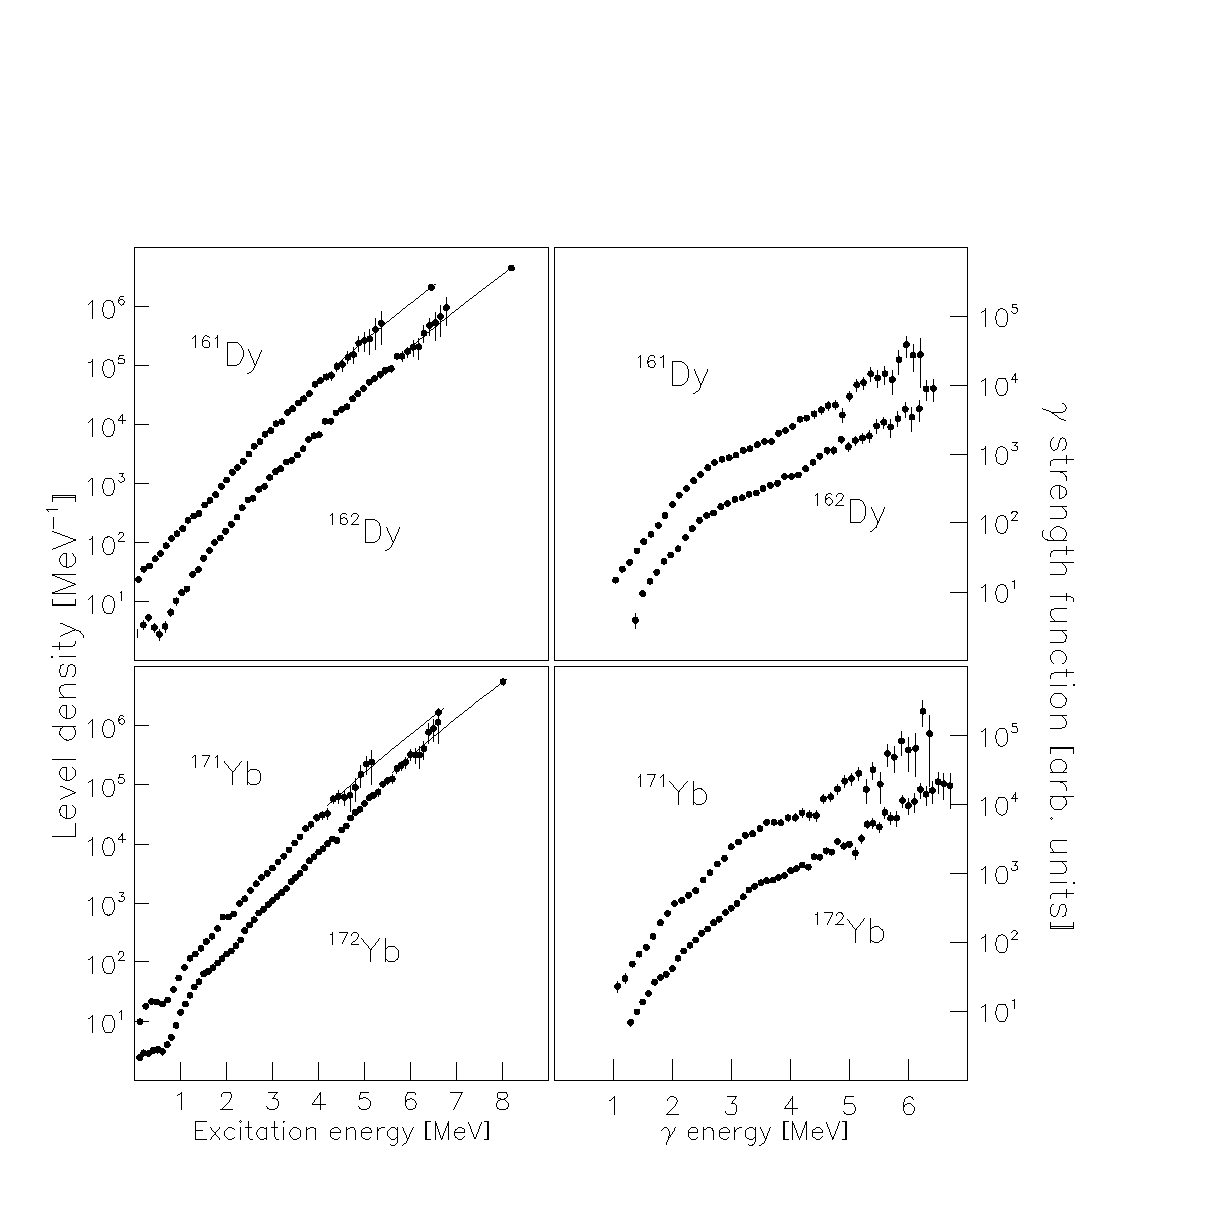
\includegraphics[totalheight=17.9cm]{fig1.eps}
\caption{Experimental level density (points in left panels) and $\gamma$ 
strength function (right panels) for $^{161,162}$Dy (upper part) and 
$^{171,172}$Yb (lower part). The error bars show the statistical uncertainties.
The solid lines are extrapolations based on a shifted Fermi gas model (see 
text). The isolated point at the neutron binding energy is obtained from 
neutron resonance spacing data.}
\label{fig:leveldensity}
\end{figure}

\clearpage

\begin{figure}\centering
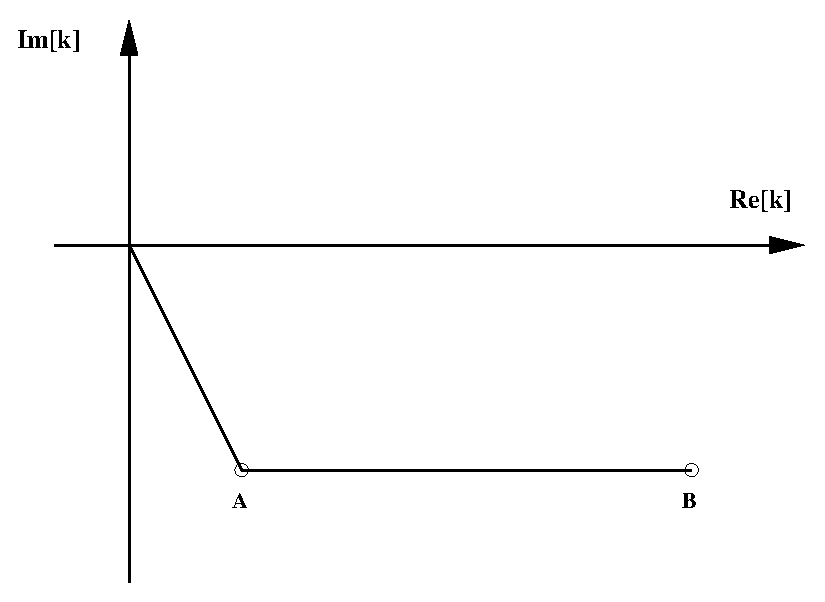
\includegraphics[totalheight=21.5cm]{fig2.eps}
\caption{Semi-experimental heat capacity as function of temperature (left 
panels) and energy $\langle E\rangle$ (right panels) in the canonical ensemble 
for $^{161,162}$Dy and $^{171,172}$Yb. The dashed lines describe the 
approximate Fermi gas heat capacity. The arrows indicate the first local 
maxima of the experimental curve relative to the Fermi gas estimates. The 
dashed dotted lines describe estimates according to Eq.~(\protect{\ref{eq:Tc}})
where $\tau$ is set equal to the critical temperature $T_c$. $T_c$ is indicated
by the vertical lines.}
\label{fig:heatcapacity} 
\end{figure}

\clearpage

\begin{figure}\centering
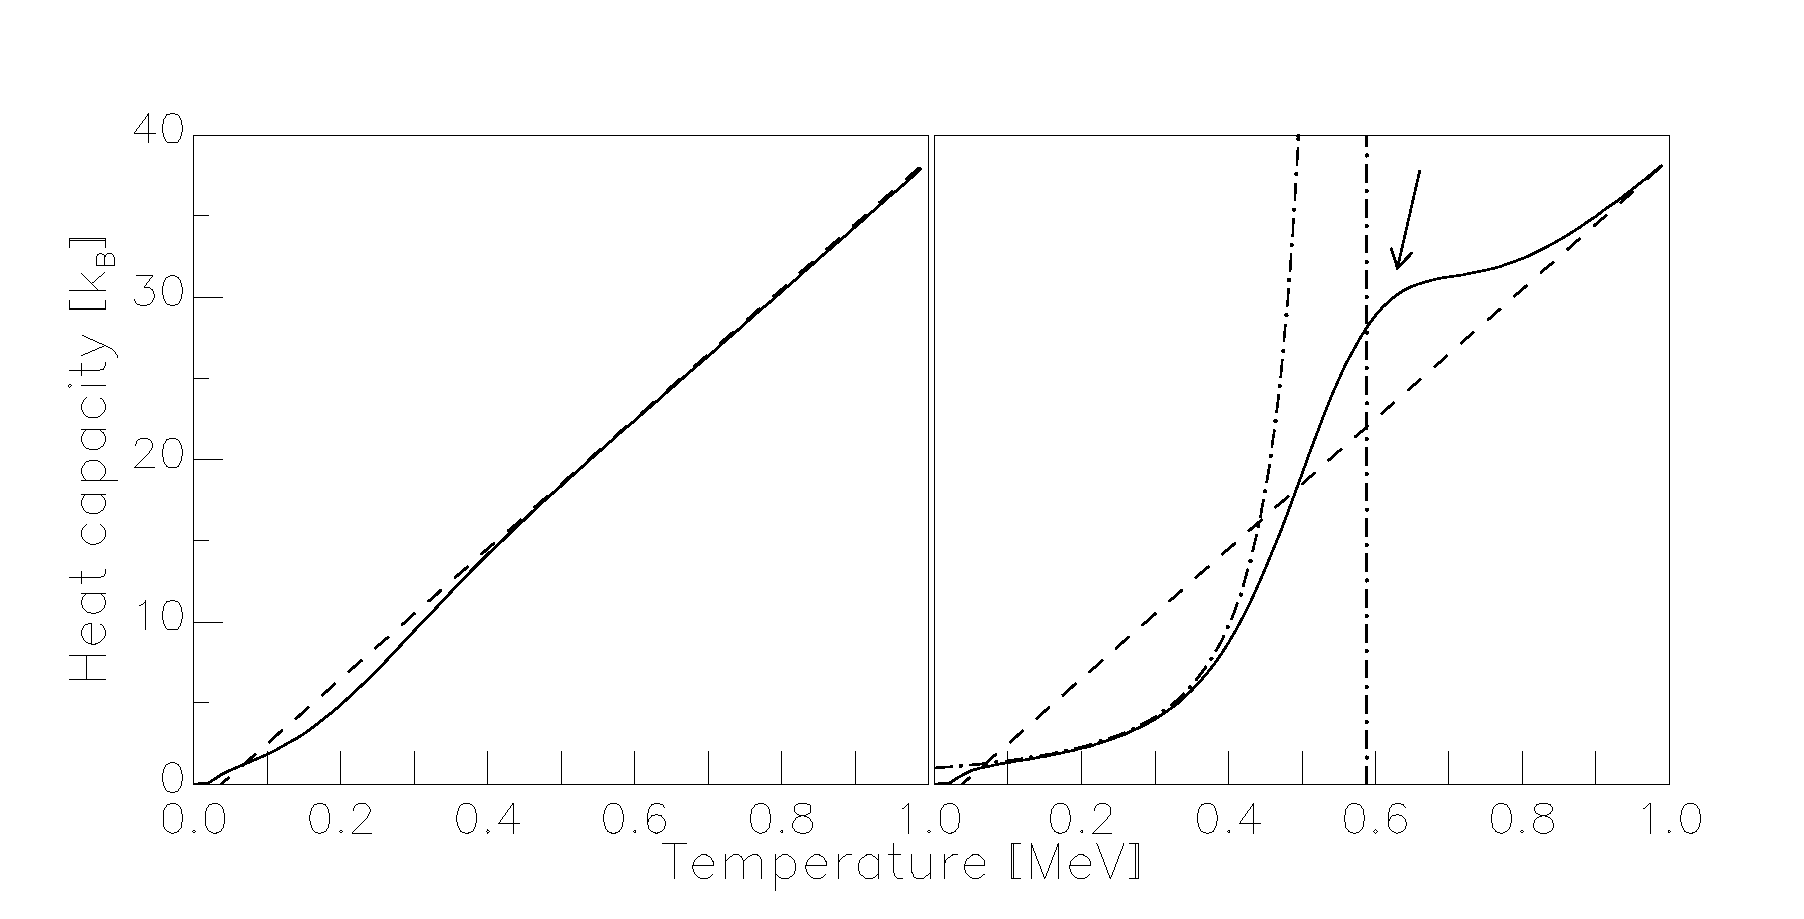
\includegraphics[totalheight=8.9cm]{fig3.eps}
\caption{A pure Fermi gas model cannot give rise to the characteristic S-shape
of the canonical heat capacity curve $C_V(T)$ (left panel). A simple composite
level density can simulate our experimental findings (right panel).}
\label{fig:simulation} 
\end{figure}

\clearpage

\begin{figure}\centering
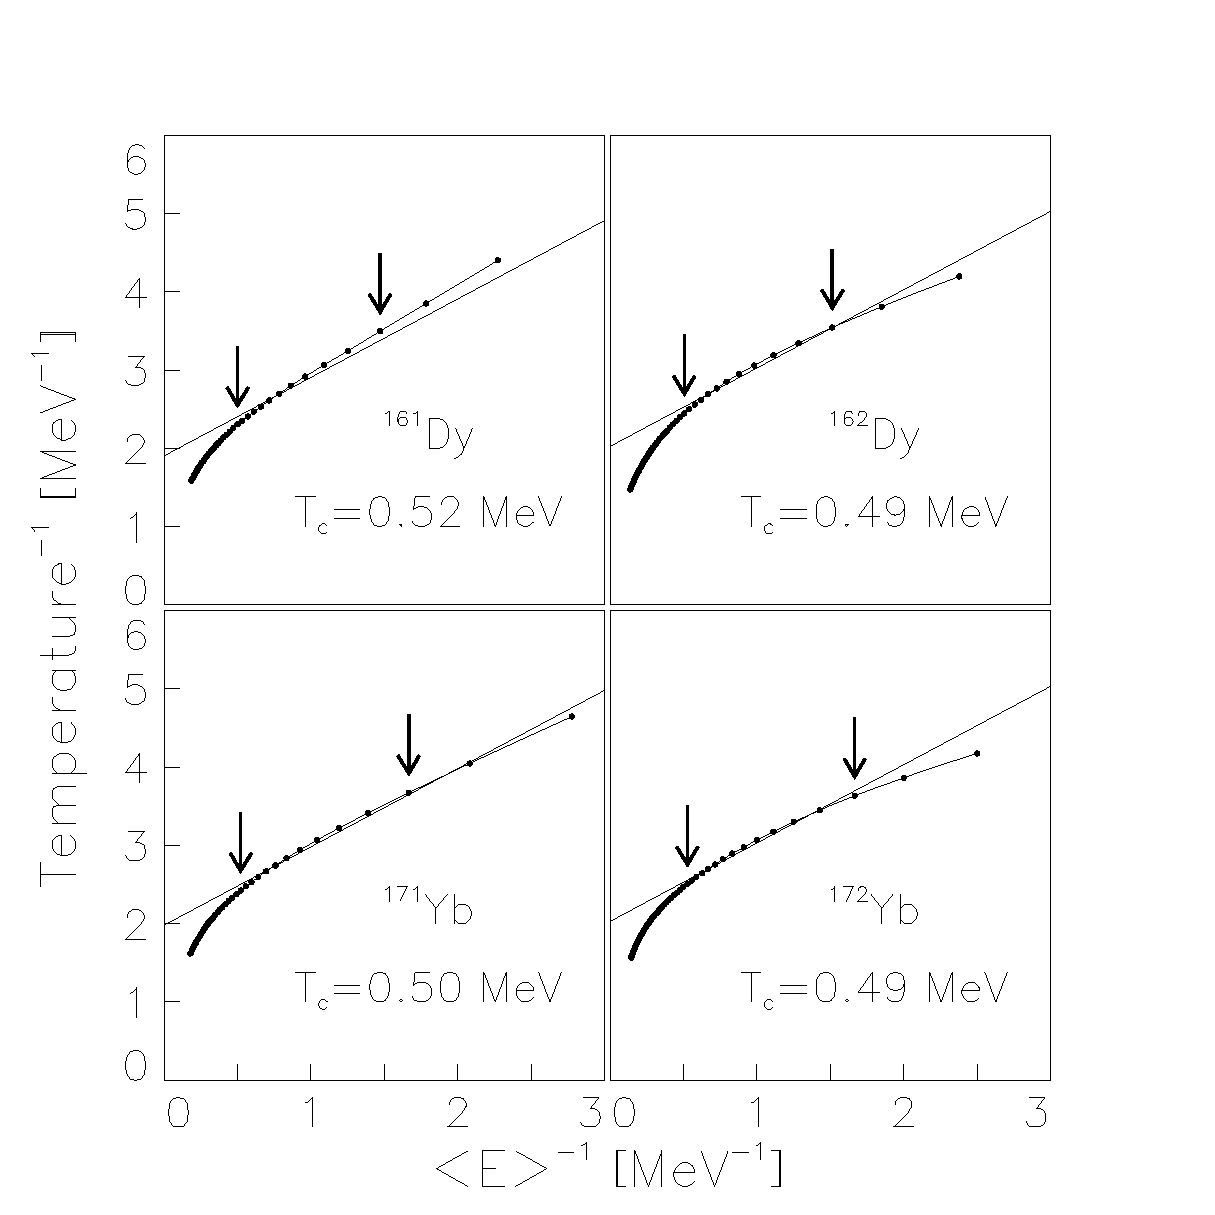
\includegraphics[totalheight=17.9cm]{fig4.eps}
\caption{The critical temperature is deduced by fitting a straight line with 
slope 1 to the data points between the arrows.}
\label{fig:critical} 
\end{figure}

\end{document}

